\documentclass[1p]{elsarticle_modified}
%\bibliographystyle{elsarticle-num}

%\usepackage[colorlinks]{hyperref}
%\usepackage{abbrmath_seonhwa} %\Abb, \Ascr, \Acal ,\Abf, \Afrak
\usepackage{amsfonts}
\usepackage{amssymb}
\usepackage{amsmath}
\usepackage{amsthm}
\usepackage{scalefnt}
\usepackage{amsbsy}
\usepackage{kotex}
\usepackage{caption}
\usepackage{subfig}
\usepackage{color}
\usepackage{graphicx}
\usepackage{xcolor} %% white, black, red, green, blue, cyan, magenta, yellow
\usepackage{float}
\usepackage{setspace}
\usepackage{hyperref}

\usepackage{tikz}
\usetikzlibrary{arrows}

\usepackage{multirow}
\usepackage{array} % fixed length table
\usepackage{hhline}

%%%%%%%%%%%%%%%%%%%%%
\makeatletter
\renewcommand*\env@matrix[1][\arraystretch]{%
	\edef\arraystretch{#1}%
	\hskip -\arraycolsep
	\let\@ifnextchar\new@ifnextchar
	\array{*\c@MaxMatrixCols c}}
\makeatother %https://tex.stackexchange.com/questions/14071/how-can-i-increase-the-line-spacing-in-a-matrix
%%%%%%%%%%%%%%%

\usepackage[normalem]{ulem}

\newcommand{\msout}[1]{\ifmmode\text{\sout{\ensuremath{#1}}}\else\sout{#1}\fi}
%SOURCE: \msout is \stkout macro in https://tex.stackexchange.com/questions/20609/strikeout-in-math-mode

\newcommand{\cancel}[1]{
	\ifmmode
	{\color{red}\msout{#1}}
	\else
	{\color{red}\sout{#1}}
	\fi
}

\newcommand{\add}[1]{
	{\color{blue}\uwave{#1}}
}

\newcommand{\replace}[2]{
	\ifmmode
	{\color{red}\msout{#1}}{\color{blue}\uwave{#2}}
	\else
	{\color{red}\sout{#1}}{\color{blue}\uwave{#2}}
	\fi
}

\newcommand{\Sol}{\mathcal{S}} %segment
\newcommand{\D}{D} %diagram
\newcommand{\A}{\mathcal{A}} %arc


%%%%%%%%%%%%%%%%%%%%%%%%%%%%%5 test

\def\sl{\operatorname{\textup{SL}}(2,\Cbb)}
\def\psl{\operatorname{\textup{PSL}}(2,\Cbb)}
\def\quan{\mkern 1mu \triangleright \mkern 1mu}

\theoremstyle{definition}
\newtheorem{thm}{Theorem}[section]
\newtheorem{prop}[thm]{Proposition}
\newtheorem{lem}[thm]{Lemma}
\newtheorem{ques}[thm]{Question}
\newtheorem{cor}[thm]{Corollary}
\newtheorem{defn}[thm]{Definition}
\newtheorem{exam}[thm]{Example}
\newtheorem{rmk}[thm]{Remark}
\newtheorem{alg}[thm]{Algorithm}

\newcommand{\I}{\sqrt{-1}}
\begin{document}

%\begin{frontmatter}
%
%\title{Boundary parabolic representations of knots up to 8 crossings}
%
%%% Group authors per affiliation:
%\author{Yunhi Cho} 
%\address{Department of Mathematics, University of Seoul, Seoul, Korea}
%\ead{yhcho@uos.ac.kr}
%
%
%\author{Seonhwa Kim} %\fnref{s_kim}}
%\address{Center for Geometry and Physics, Institute for Basic Science, Pohang, 37673, Korea}
%\ead{ryeona17@ibs.re.kr}
%
%\author{Hyuk Kim}
%\address{Department of Mathematical Sciences, Seoul National University, Seoul 08826, Korea}
%\ead{hyukkim@snu.ac.kr}
%
%\author{Seokbeom Yoon}
%\address{Department of Mathematical Sciences, Seoul National University, Seoul, 08826,  Korea}
%\ead{sbyoon15@snu.ac.kr}
%
%\begin{abstract}
%We find all boundary parabolic representation of knots up to 8 crossings.
%
%\end{abstract}
%\begin{keyword}
%    \MSC[2010] 57M25 
%\end{keyword}
%
%\end{frontmatter}

%\linenumbers
%\tableofcontents
%
\newcommand\colored[1]{\textcolor{white}{\rule[-0.35ex]{0.8em}{1.4ex}}\kern-0.8em\color{red} #1}%
%\newcommand\colored[1]{\textcolor{white}{ #1}\kern-2.17ex	\textcolor{white}{ #1}\kern-1.81ex	\textcolor{white}{ #1}\kern-2.15ex\color{red}#1	}

{\Large $\underline{10_{89}~(K10a_{21})}$}

\setlength{\tabcolsep}{10pt}
\renewcommand{\arraystretch}{1.6}
\vspace{1cm}\begin{tabular}{m{100pt}>{\centering\arraybackslash}m{274pt}}
\multirow{5}{120pt}{
	\centering
	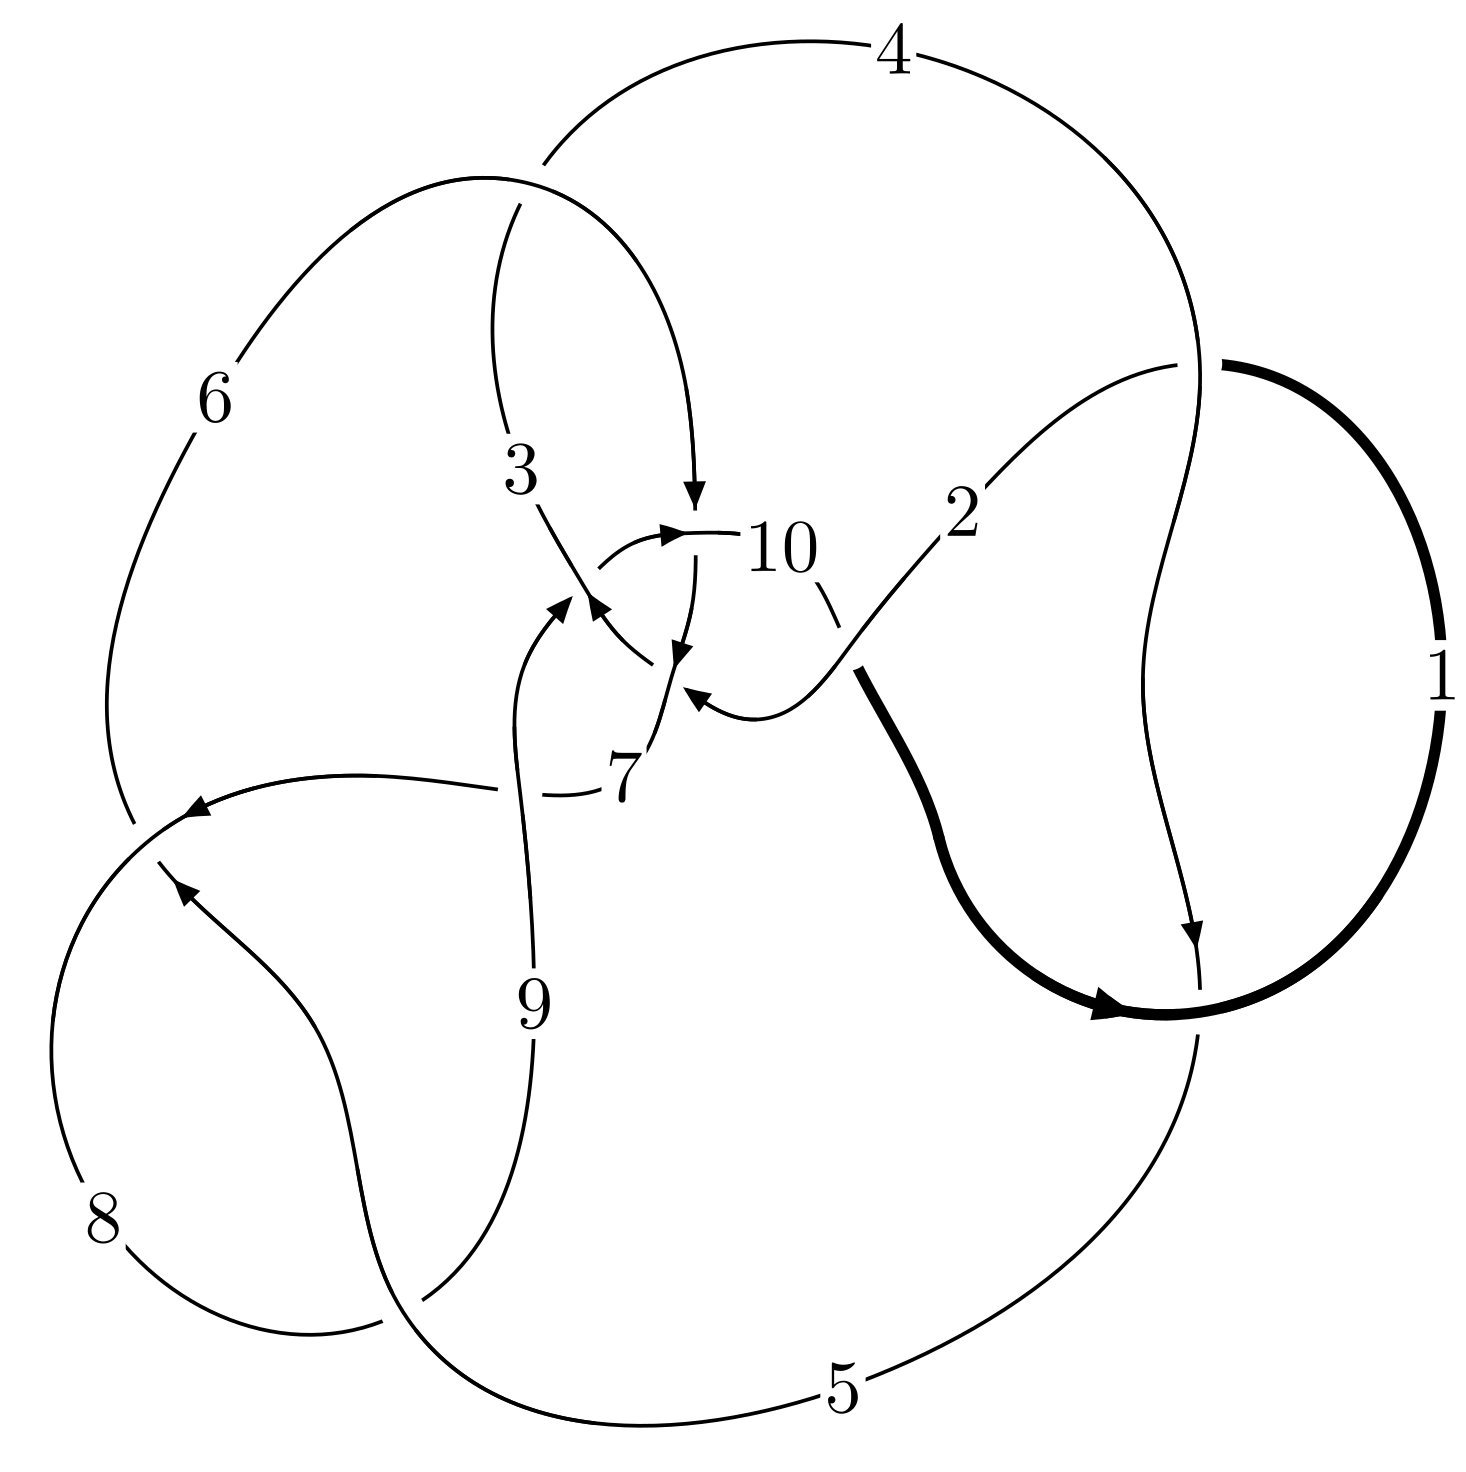
\includegraphics[width=112pt]{../../../GIT/diagram.site/Diagrams/png/173_10_89.png}\\
\ \ \ A knot diagram\footnotemark}&
\allowdisplaybreaks
\textbf{Linearized knot diagam} \\
\cline{2-2}
 &
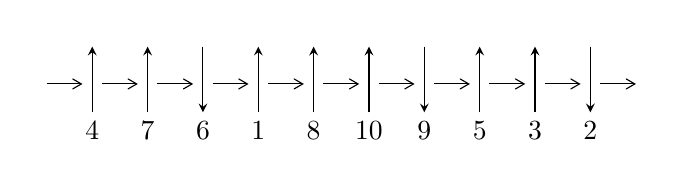
\begin{tikzpicture}[x=20pt, y=17pt]
	% nodes
	\node (C0) at (0, 0) {};
	\node (C1) at (1, 0) {};
	\node (C1U) at (1, +1) {};
	\node (C1D) at (1, -1) {4};

	\node (C2) at (2, 0) {};
	\node (C2U) at (2, +1) {};
	\node (C2D) at (2, -1) {7};

	\node (C3) at (3, 0) {};
	\node (C3U) at (3, +1) {};
	\node (C3D) at (3, -1) {6};

	\node (C4) at (4, 0) {};
	\node (C4U) at (4, +1) {};
	\node (C4D) at (4, -1) {1};

	\node (C5) at (5, 0) {};
	\node (C5U) at (5, +1) {};
	\node (C5D) at (5, -1) {8};

	\node (C6) at (6, 0) {};
	\node (C6U) at (6, +1) {};
	\node (C6D) at (6, -1) {10};

	\node (C7) at (7, 0) {};
	\node (C7U) at (7, +1) {};
	\node (C7D) at (7, -1) {9};

	\node (C8) at (8, 0) {};
	\node (C8U) at (8, +1) {};
	\node (C8D) at (8, -1) {5};

	\node (C9) at (9, 0) {};
	\node (C9U) at (9, +1) {};
	\node (C9D) at (9, -1) {3};

	\node (C10) at (10, 0) {};
	\node (C10U) at (10, +1) {};
	\node (C10D) at (10, -1) {2};
	\node (C11) at (11, 0) {};

	% arrows
	\draw[->,>={angle 60}]
	(C0) edge (C1) (C1) edge (C2) (C2) edge (C3) (C3) edge (C4) (C4) edge (C5) (C5) edge (C6) (C6) edge (C7) (C7) edge (C8) (C8) edge (C9) (C9) edge (C10) (C10) edge (C11) ;	\draw[->,>=stealth]
	(C1D) edge (C1U) (C2D) edge (C2U) (C3U) edge (C3D) (C4D) edge (C4U) (C5D) edge (C5U) (C6D) edge (C6U) (C7U) edge (C7D) (C8D) edge (C8U) (C9D) edge (C9U) (C10U) edge (C10D) ;
	\end{tikzpicture} \\
\hhline{~~} \\& 
\textbf{Solving Sequence} \\ \cline{2-2} 
 &
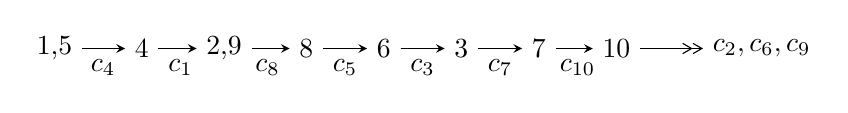
\begin{tikzpicture}[x=28pt, y=7pt]
	% node
	\node (A0) at (-1/8, 0) {1,5};
	\node (A1) at (1, 0) {4};
	\node (A2) at (33/16, 0) {2,9};
	\node (A3) at (25/8, 0) {8};
	\node (A4) at (33/8, 0) {6};
	\node (A5) at (41/8, 0) {3};
	\node (A6) at (49/8, 0) {7};
	\node (A7) at (57/8, 0) {10};
	\node (C1) at (1/2, -1) {$c_{4}$};
	\node (C2) at (3/2, -1) {$c_{1}$};
	\node (C3) at (21/8, -1) {$c_{8}$};
	\node (C4) at (29/8, -1) {$c_{5}$};
	\node (C5) at (37/8, -1) {$c_{3}$};
	\node (C6) at (45/8, -1) {$c_{7}$};
	\node (C7) at (53/8, -1) {$c_{10}$};
	\node (A8) at (9, 0) {$c_{2},c_{6},c_{9}$};

	% edge
	\draw[->,>=stealth]	
	(A0) edge (A1) (A1) edge (A2) (A2) edge (A3) (A3) edge (A4) (A4) edge (A5) (A5) edge (A6) (A6) edge (A7) ;
	\draw[->>,>={angle 60}]	
	(A7) edge (A8);
\end{tikzpicture} \\ 

\end{tabular} \\

\footnotetext{
The image of knot diagram is generated by the software ``\textbf{Draw programme}" developed by Andrew Bartholomew(\url{http://www.layer8.co.uk/maths/draw/index.htm\#Running-draw}), where we modified some parts for our purpose(\url{https://github.com/CATsTAILs/LinksPainter}).
}\phantom \\ \newline 
\centering \textbf{Ideals for irreducible components\footnotemark of $X_{\text{par}}$} 
 
\begin{align*}
I^u_{1}&=\langle 
b+u,\;u^8+2 u^7+3 u^6+2 u^5+u^4+a-1,\;u^9+2 u^8+4 u^7+4 u^6+5 u^5+4 u^4+4 u^3+2 u^2+u-1\rangle \\
I^u_{2}&=\langle 
-2.54158\times10^{21} u^{39}+3.72578\times10^{21} u^{38}+\cdots+1.43109\times10^{22} b-1.56356\times10^{21},\\
\phantom{I^u_{2}}&\phantom{= \langle  }-3.70291\times10^{21} u^{39}+3.38172\times10^{21} u^{38}+\cdots+1.43109\times10^{22} a-2.35738\times10^{22},\;u^{40}- u^{39}+\cdots-4 u+1\rangle \\
\\
\end{align*}
\raggedright * 2 irreducible components of $\dim_{\mathbb{C}}=0$, with total 49 representations.\\
\footnotetext{All coefficients of polynomials are rational numbers. But the coefficients are sometimes approximated in decimal forms when there is not enough margin.}
\newpage
\renewcommand{\arraystretch}{1}
\centering \section*{I. $I^u_{1}= \langle b+u,\;u^8+2 u^7+3 u^6+2 u^5+u^4+a-1,\;u^9+2 u^8+\cdots+u-1 \rangle$}
\flushleft \textbf{(i) Arc colorings}\\
\begin{tabular}{m{7pt} m{180pt} m{7pt} m{180pt} }
\flushright $a_{1}=$&$\begin{pmatrix}0\\u\end{pmatrix}$ \\
\flushright $a_{5}=$&$\begin{pmatrix}1\\0\end{pmatrix}$ \\
\flushright $a_{4}=$&$\begin{pmatrix}1\\u^2\end{pmatrix}$ \\
\flushright $a_{2}=$&$\begin{pmatrix}u\\u^3+u\end{pmatrix}$ \\
\flushright $a_{9}=$&$\begin{pmatrix}- u^8-2 u^7-3 u^6-2 u^5- u^4+1\\- u\end{pmatrix}$ \\
\flushright $a_{8}=$&$\begin{pmatrix}- u^8-2 u^7-3 u^6-2 u^5- u^4+u+1\\- u\end{pmatrix}$ \\
\flushright $a_{6}=$&$\begin{pmatrix}u^7+2 u^6+4 u^5+4 u^4+4 u^3+3 u^2+2 u\\- u^2\end{pmatrix}$ \\
\flushright $a_{3}=$&$\begin{pmatrix}u^7+3 u^6+7 u^5+8 u^4+7 u^3+4 u^2+u\\u^7+u^6+2 u^5+u^4+u^3\end{pmatrix}$ \\
\flushright $a_{7}=$&$\begin{pmatrix}u^6+2 u^5+3 u^4+2 u^3+2 u^2+1\\- u^3- u\end{pmatrix}$ \\
\flushright $a_{10}=$&$\begin{pmatrix}u^3\\u^5+u^3+u\end{pmatrix}$\\&\end{tabular}
\flushleft \textbf{(ii) Obstruction class $= -1$}\\~\\
\flushleft \textbf{(iii) Cusp Shapes $= -4 u^8-4 u^7-8 u^6-4 u^5-4 u^4+4 u^3+8 u^2+8 u+6$}\\~\\
\newpage\renewcommand{\arraystretch}{1}
\flushleft \textbf{(iv) u-Polynomials at the component}\newline \\
\begin{tabular}{m{50pt}|m{274pt}}
Crossings & \hspace{64pt}u-Polynomials at each crossing \\
\hline $$\begin{aligned}c_{1},c_{4},c_{5}\\c_{8}\end{aligned}$$&$\begin{aligned}
&u^9+2 u^8+4 u^7+4 u^6+5 u^5+4 u^4+4 u^3+2 u^2+u-1
\end{aligned}$\\
\hline $$\begin{aligned}c_{2}\end{aligned}$$&$\begin{aligned}
&u^9-13 u^8+\cdots+152 u-32
\end{aligned}$\\
\hline $$\begin{aligned}c_{3}\end{aligned}$$&$\begin{aligned}
&u^9-13 u^8+\cdots+208 u-32
\end{aligned}$\\
\hline $$\begin{aligned}c_{6},c_{9}\end{aligned}$$&$\begin{aligned}
&u^9-2 u^6+5 u^5+4 u^3-6 u^2+3 u-1
\end{aligned}$\\
\hline $$\begin{aligned}c_{7},c_{10}\end{aligned}$$&$\begin{aligned}
&u^9+4 u^8+10 u^7+16 u^6+19 u^5+20 u^4+18 u^3+12 u^2+5 u-1
\end{aligned}$\\
\hline
\end{tabular}\\~\\
\newpage\renewcommand{\arraystretch}{1}
\flushleft \textbf{(v) Riley Polynomials at the component}\newline \\
\begin{tabular}{m{50pt}|m{274pt}}
Crossings & \hspace{64pt}Riley Polynomials at each crossing \\
\hline $$\begin{aligned}c_{1},c_{4},c_{5}\\c_{8}\end{aligned}$$&$\begin{aligned}
&y^9+4 y^8+10 y^7+16 y^6+19 y^5+20 y^4+18 y^3+12 y^2+5 y-1
\end{aligned}$\\
\hline $$\begin{aligned}c_{2}\end{aligned}$$&$\begin{aligned}
&y^9-25 y^8+\cdots-192 y-1024
\end{aligned}$\\
\hline $$\begin{aligned}c_{3}\end{aligned}$$&$\begin{aligned}
&y^9-23 y^8+\cdots+8960 y-1024
\end{aligned}$\\
\hline $$\begin{aligned}c_{6},c_{9}\end{aligned}$$&$\begin{aligned}
&y^9+10 y^7+4 y^6+31 y^5+16 y^4+42 y^3-12 y^2-3 y-1
\end{aligned}$\\
\hline $$\begin{aligned}c_{7},c_{10}\end{aligned}$$&$\begin{aligned}
&y^9+4 y^8+10 y^7-5 y^5+8 y^4+66 y^3+76 y^2+49 y-1
\end{aligned}$\\
\hline
\end{tabular}\\~\\
\newpage\flushleft \textbf{(vi) Complex Volumes and Cusp Shapes}
$$\begin{array}{c|c|c}  
\text{Solutions to }I^u_{1}& \I (\text{vol} + \sqrt{-1}CS) & \text{Cusp shape}\\
 \hline 
\begin{aligned}
u &= -0.870256 + 0.574591 I \\
a &= \phantom{-}1.51055 - 0.27719 I \\
b &= \phantom{-}0.870256 - 0.574591 I\end{aligned}
 & \phantom{-}4.84938 + 3.79988 I & \phantom{-}8.45408 - 1.48636 I \\ \hline\begin{aligned}
u &= -0.870256 - 0.574591 I \\
a &= \phantom{-}1.51055 + 0.27719 I \\
b &= \phantom{-}0.870256 + 0.574591 I\end{aligned}
 & \phantom{-}4.84938 - 3.79988 I & \phantom{-}8.45408 + 1.48636 I \\ \hline\begin{aligned}
u &= \phantom{-}0.547196 + 0.894013 I \\
a &= -4.54039 + 0.41851 I \\
b &= -0.547196 - 0.894013 I\end{aligned}
 & \phantom{-}0.19748 + 4.39098 I & -9.5886 + 15.7654 I \\ \hline\begin{aligned}
u &= \phantom{-}0.547196 - 0.894013 I \\
a &= -4.54039 - 0.41851 I \\
b &= -0.547196 + 0.894013 I\end{aligned}
 & \phantom{-}0.19748 - 4.39098 I & -9.5886 - 15.7654 I \\ \hline\begin{aligned}
u &= -0.168491 + 1.118820 I \\
a &= \phantom{-}1.00104 + 1.15340 I \\
b &= \phantom{-}0.168491 - 1.118820 I\end{aligned}
 & -6.19752 + 0.38154 I & -4.67885 - 0.54411 I \\ \hline\begin{aligned}
u &= -0.168491 - 1.118820 I \\
a &= \phantom{-}1.00104 - 1.15340 I \\
b &= \phantom{-}0.168491 + 1.118820 I\end{aligned}
 & -6.19752 - 0.38154 I & -4.67885 + 0.54411 I \\ \hline\begin{aligned}
u &= -0.695984 + 1.121930 I \\
a &= \phantom{-}2.05153 + 0.69357 I \\
b &= \phantom{-}0.695984 - 1.121930 I\end{aligned}
 & \phantom{-}1.4591 - 15.5661 I & \phantom{-}3.71332 + 9.69859 I \\ \hline\begin{aligned}
u &= -0.695984 - 1.121930 I \\
a &= \phantom{-}2.05153 - 0.69357 I \\
b &= \phantom{-}0.695984 + 1.121930 I\end{aligned}
 & \phantom{-}1.4591 + 15.5661 I & \phantom{-}3.71332 - 9.69859 I \\ \hline\begin{aligned}
u &= \phantom{-}0.375070\phantom{ +0.000000I} \\
a &= \phantom{-}0.954532\phantom{ +0.000000I} \\
b &= -0.375070\phantom{ +0.000000I}\end{aligned}
 & \phantom{-}1.02805\phantom{ +0.000000I} & \phantom{-}10.2000\phantom{ +0.000000I}\\
 \hline 
 \end{array}$$\newpage\newpage\renewcommand{\arraystretch}{1}
\centering \section*{II. $I^u_{2}= \langle -2.54\times10^{21} u^{39}+3.73\times10^{21} u^{38}+\cdots+1.43\times10^{22} b-1.56\times10^{21},\;-3.70\times10^{21} u^{39}+3.38\times10^{21} u^{38}+\cdots+1.43\times10^{22} a-2.36\times10^{22},\;u^{40}- u^{39}+\cdots-4 u+1 \rangle$}
\flushleft \textbf{(i) Arc colorings}\\
\begin{tabular}{m{7pt} m{180pt} m{7pt} m{180pt} }
\flushright $a_{1}=$&$\begin{pmatrix}0\\u\end{pmatrix}$ \\
\flushright $a_{5}=$&$\begin{pmatrix}1\\0\end{pmatrix}$ \\
\flushright $a_{4}=$&$\begin{pmatrix}1\\u^2\end{pmatrix}$ \\
\flushright $a_{2}=$&$\begin{pmatrix}u\\u^3+u\end{pmatrix}$ \\
\flushright $a_{9}=$&$\begin{pmatrix}0.258747 u^{39}-0.236304 u^{38}+\cdots-1.86737 u+1.64726\\0.177597 u^{39}-0.260346 u^{38}+\cdots-3.36976 u+0.109256\end{pmatrix}$ \\
\flushright $a_{8}=$&$\begin{pmatrix}0.0811501 u^{39}+0.0240417 u^{38}+\cdots+1.50239 u+1.53800\\0.177597 u^{39}-0.260346 u^{38}+\cdots-3.36976 u+0.109256\end{pmatrix}$ \\
\flushright $a_{6}=$&$\begin{pmatrix}-0.0521006 u^{39}-0.686202 u^{38}+\cdots+4.91261 u+0.428336\\0.110686 u^{39}-0.236069 u^{38}+\cdots-3.29989 u+1.06601\end{pmatrix}$ \\
\flushright $a_{3}=$&$\begin{pmatrix}1.44465 u^{39}-1.15627 u^{38}+\cdots+1.62073 u-1.83432\\0.138363 u^{39}+0.574052 u^{38}+\cdots+2.22447 u+0.383801\end{pmatrix}$ \\
\flushright $a_{7}=$&$\begin{pmatrix}-0.00240648 u^{39}-0.744206 u^{38}+\cdots+4.44922 u+0.596332\\0.0437786 u^{39}-0.281347 u^{38}+\cdots-3.16226 u+1.11303\end{pmatrix}$ \\
\flushright $a_{10}=$&$\begin{pmatrix}u^3\\u^5+u^3+u\end{pmatrix}$\\&\end{tabular}
\flushleft \textbf{(ii) Obstruction class $= -1$}\\~\\
\flushleft \textbf{(iii) Cusp Shapes $= \frac{72408804377930288848424}{14310892564212518359243} u^{39}-\frac{77968614159801719652396}{14310892564212518359243} u^{38}+\cdots-\frac{8681622498642290526880}{622212720183152972141} u+\frac{76038785248810355101710}{14310892564212518359243}$}\\~\\
\newpage\renewcommand{\arraystretch}{1}
\flushleft \textbf{(iv) u-Polynomials at the component}\newline \\
\begin{tabular}{m{50pt}|m{274pt}}
Crossings & \hspace{64pt}u-Polynomials at each crossing \\
\hline $$\begin{aligned}c_{1},c_{4},c_{5}\\c_{8}\end{aligned}$$&$\begin{aligned}
&u^{40}- u^{39}+\cdots-4 u+1
\end{aligned}$\\
\hline $$\begin{aligned}c_{2}\end{aligned}$$&$\begin{aligned}
&(u^{20}+6 u^{19}+\cdots-2 u-1)^{2}
\end{aligned}$\\
\hline $$\begin{aligned}c_{3}\end{aligned}$$&$\begin{aligned}
&(u^{20}+5 u^{19}+\cdots-6 u-1)^{2}
\end{aligned}$\\
\hline $$\begin{aligned}c_{6},c_{9}\end{aligned}$$&$\begin{aligned}
&u^{40}+5 u^{39}+\cdots+4 u+1
\end{aligned}$\\
\hline $$\begin{aligned}c_{7},c_{10}\end{aligned}$$&$\begin{aligned}
&u^{40}+15 u^{39}+\cdots+120 u^2+1
\end{aligned}$\\
\hline
\end{tabular}\\~\\
\newpage\renewcommand{\arraystretch}{1}
\flushleft \textbf{(v) Riley Polynomials at the component}\newline \\
\begin{tabular}{m{50pt}|m{274pt}}
Crossings & \hspace{64pt}Riley Polynomials at each crossing \\
\hline $$\begin{aligned}c_{1},c_{4},c_{5}\\c_{8}\end{aligned}$$&$\begin{aligned}
&y^{40}+15 y^{39}+\cdots+120 y^2+1
\end{aligned}$\\
\hline $$\begin{aligned}c_{2}\end{aligned}$$&$\begin{aligned}
&(y^{20}-16 y^{19}+\cdots-16 y+1)^{2}
\end{aligned}$\\
\hline $$\begin{aligned}c_{3}\end{aligned}$$&$\begin{aligned}
&(y^{20}-7 y^{19}+\cdots-2 y+1)^{2}
\end{aligned}$\\
\hline $$\begin{aligned}c_{6},c_{9}\end{aligned}$$&$\begin{aligned}
&y^{40}-5 y^{39}+\cdots-8 y+1
\end{aligned}$\\
\hline $$\begin{aligned}c_{7},c_{10}\end{aligned}$$&$\begin{aligned}
&y^{40}+19 y^{39}+\cdots+240 y+1
\end{aligned}$\\
\hline
\end{tabular}\\~\\
\newpage\flushleft \textbf{(vi) Complex Volumes and Cusp Shapes}
$$\begin{array}{c|c|c}  
\text{Solutions to }I^u_{2}& \I (\text{vol} + \sqrt{-1}CS) & \text{Cusp shape}\\
 \hline 
\begin{aligned}
u &= \phantom{-}0.548393 + 0.820650 I \\
a &= -1.93438 + 2.89472 I \\
b &= -0.548393 + 0.820650 I\end{aligned}
 & \phantom{-}0.434649\phantom{ +0.000000I} & -15.8981 + 0. I\phantom{ +0.000000I} \\ \hline\begin{aligned}
u &= \phantom{-}0.548393 - 0.820650 I \\
a &= -1.93438 - 2.89472 I \\
b &= -0.548393 - 0.820650 I\end{aligned}
 & \phantom{-}0.434649\phantom{ +0.000000I} & -15.8981 + 0. I\phantom{ +0.000000I} \\ \hline\begin{aligned}
u &= -0.632900 + 0.810710 I \\
a &= -0.713489 - 1.128410 I \\
b &= -1.003700 - 0.392952 I\end{aligned}
 & \phantom{-}3.51067 - 0.70102 I & \phantom{-}13.30095 + 0.29053 I \\ \hline\begin{aligned}
u &= -0.632900 - 0.810710 I \\
a &= -0.713489 + 1.128410 I \\
b &= -1.003700 + 0.392952 I\end{aligned}
 & \phantom{-}3.51067 + 0.70102 I & \phantom{-}13.30095 - 0.29053 I \\ \hline\begin{aligned}
u &= \phantom{-}0.602510 + 0.849943 I \\
a &= \phantom{-}0.252963 - 0.117129 I \\
b &= -0.232545 - 0.154995 I\end{aligned}
 & \phantom{-}0.59509 + 2.36716 I & \phantom{-}1.43169 - 3.69296 I \\ \hline\begin{aligned}
u &= \phantom{-}0.602510 - 0.849943 I \\
a &= \phantom{-}0.252963 + 0.117129 I \\
b &= -0.232545 + 0.154995 I\end{aligned}
 & \phantom{-}0.59509 - 2.36716 I & \phantom{-}1.43169 + 3.69296 I \\ \hline\begin{aligned}
u &= \phantom{-}0.378614 + 0.869397 I \\
a &= \phantom{-}1.02843 - 2.36154 I \\
b &= -0.378614 + 0.869397 I\end{aligned}
 & -0.714628\phantom{ +0.000000I} & \phantom{-}8.43291 + 0. I\phantom{ +0.000000I} \\ \hline\begin{aligned}
u &= \phantom{-}0.378614 - 0.869397 I \\
a &= \phantom{-}1.02843 + 2.36154 I \\
b &= -0.378614 - 0.869397 I\end{aligned}
 & -0.714628\phantom{ +0.000000I} & \phantom{-}8.43291 + 0. I\phantom{ +0.000000I} \\ \hline\begin{aligned}
u &= -0.932276 + 0.516877 I \\
a &= \phantom{-}1.277650 + 0.549417 I \\
b &= \phantom{-}0.693643 + 1.075960 I\end{aligned}
 & \phantom{-}3.31734 + 9.59937 I & \phantom{-}6.13875 - 5.98964 I \\ \hline\begin{aligned}
u &= -0.932276 - 0.516877 I \\
a &= \phantom{-}1.277650 - 0.549417 I \\
b &= \phantom{-}0.693643 - 1.075960 I\end{aligned}
 & \phantom{-}3.31734 - 9.59937 I & \phantom{-}6.13875 + 5.98964 I\\
 \hline 
 \end{array}$$\newpage$$\begin{array}{c|c|c}  
\text{Solutions to }I^u_{2}& \I (\text{vol} + \sqrt{-1}CS) & \text{Cusp shape}\\
 \hline 
\begin{aligned}
u &= -0.592803 + 0.720077 I \\
a &= -0.714830 - 0.969785 I \\
b &= -0.783556 - 1.064140 I\end{aligned}
 & \phantom{-}1.83047 + 2.21575 I & \phantom{-}9.27050 - 4.60917 I \\ \hline\begin{aligned}
u &= -0.592803 - 0.720077 I \\
a &= -0.714830 + 0.969785 I \\
b &= -0.783556 + 1.064140 I\end{aligned}
 & \phantom{-}1.83047 - 2.21575 I & \phantom{-}9.27050 + 4.60917 I \\ \hline\begin{aligned}
u &= -0.630140 + 0.869793 I \\
a &= -1.50017 - 0.30493 I \\
b &= -1.009240 + 0.568343 I\end{aligned}
 & \phantom{-}3.33020 - 4.24448 I & \phantom{-}12.4039 + 6.8707 I \\ \hline\begin{aligned}
u &= -0.630140 - 0.869793 I \\
a &= -1.50017 + 0.30493 I \\
b &= -1.009240 - 0.568343 I\end{aligned}
 & \phantom{-}3.33020 + 4.24448 I & \phantom{-}12.4039 - 6.8707 I \\ \hline\begin{aligned}
u &= \phantom{-}1.003700 + 0.392952 I \\
a &= \phantom{-}1.226320 - 0.344870 I \\
b &= \phantom{-}0.632900 - 0.810710 I\end{aligned}
 & \phantom{-}3.51067 - 0.70102 I & \phantom{-}13.30095 + 0.29053 I \\ \hline\begin{aligned}
u &= \phantom{-}1.003700 - 0.392952 I \\
a &= \phantom{-}1.226320 + 0.344870 I \\
b &= \phantom{-}0.632900 + 0.810710 I\end{aligned}
 & \phantom{-}3.51067 + 0.70102 I & \phantom{-}13.30095 - 0.29053 I \\ \hline\begin{aligned}
u &= -0.604828 + 0.939285 I \\
a &= -2.13314 - 0.62294 I \\
b &= -0.729702 + 1.179840 I\end{aligned}
 & \phantom{-}1.15558 - 6.98661 I & \phantom{-}6.87126 + 10.77467 I \\ \hline\begin{aligned}
u &= -0.604828 - 0.939285 I \\
a &= -2.13314 + 0.62294 I \\
b &= -0.729702 - 1.179840 I\end{aligned}
 & \phantom{-}1.15558 + 6.98661 I & \phantom{-}6.87126 - 10.77467 I \\ \hline\begin{aligned}
u &= \phantom{-}0.124209 + 1.127990 I \\
a &= \phantom{-}0.383349 + 0.300461 I \\
b &= \phantom{-}0.592384 - 0.373525 I\end{aligned}
 & -1.87648 + 2.61466 I & \phantom{-}1.96705 - 3.93297 I \\ \hline\begin{aligned}
u &= \phantom{-}0.124209 - 1.127990 I \\
a &= \phantom{-}0.383349 - 0.300461 I \\
b &= \phantom{-}0.592384 + 0.373525 I\end{aligned}
 & -1.87648 - 2.61466 I & \phantom{-}1.96705 + 3.93297 I\\
 \hline 
 \end{array}$$\newpage$$\begin{array}{c|c|c}  
\text{Solutions to }I^u_{2}& \I (\text{vol} + \sqrt{-1}CS) & \text{Cusp shape}\\
 \hline 
\begin{aligned}
u &= \phantom{-}0.402129 + 1.083400 I \\
a &= \phantom{-}0.297918 + 0.759573 I \\
b &= \phantom{-}0.116121 - 0.708920 I\end{aligned}
 & -1.51323 + 2.73094 I & \phantom{-}0.60746 - 4.99024 I \\ \hline\begin{aligned}
u &= \phantom{-}0.402129 - 1.083400 I \\
a &= \phantom{-}0.297918 - 0.759573 I \\
b &= \phantom{-}0.116121 + 0.708920 I\end{aligned}
 & -1.51323 - 2.73094 I & \phantom{-}0.60746 + 4.99024 I \\ \hline\begin{aligned}
u &= \phantom{-}1.009240 + 0.568343 I \\
a &= \phantom{-}1.38205 + 0.32422 I \\
b &= \phantom{-}0.630140 + 0.869793 I\end{aligned}
 & \phantom{-}3.33020 + 4.24448 I & \phantom{-}12.4039 - 6.8707 I \\ \hline\begin{aligned}
u &= \phantom{-}1.009240 - 0.568343 I \\
a &= \phantom{-}1.38205 - 0.32422 I \\
b &= \phantom{-}0.630140 - 0.869793 I\end{aligned}
 & \phantom{-}3.33020 - 4.24448 I & \phantom{-}12.4039 + 6.8707 I \\ \hline\begin{aligned}
u &= -0.575991 + 1.044940 I \\
a &= -1.005200 - 0.537066 I \\
b &= -0.056488 + 1.295430 I\end{aligned}
 & -3.62992 - 7.26942 I & -0.25897 + 8.20898 I \\ \hline\begin{aligned}
u &= -0.575991 - 1.044940 I \\
a &= -1.005200 + 0.537066 I \\
b &= -0.056488 - 1.295430 I\end{aligned}
 & -3.62992 + 7.26942 I & -0.25897 - 8.20898 I \\ \hline\begin{aligned}
u &= -0.693643 + 1.075960 I \\
a &= \phantom{-}0.527058 + 1.031180 I \\
b &= \phantom{-}0.932276 + 0.516877 I\end{aligned}
 & \phantom{-}3.31734 - 9.59937 I & \phantom{-}6.13875 + 5.98964 I \\ \hline\begin{aligned}
u &= -0.693643 - 1.075960 I \\
a &= \phantom{-}0.527058 - 1.031180 I \\
b &= \phantom{-}0.932276 - 0.516877 I\end{aligned}
 & \phantom{-}3.31734 + 9.59937 I & \phantom{-}6.13875 - 5.98964 I \\ \hline\begin{aligned}
u &= -0.116121 + 0.708920 I \\
a &= \phantom{-}1.021210 + 0.824545 I \\
b &= -0.402129 - 1.083400 I\end{aligned}
 & -1.51323 + 2.73094 I & \phantom{-}0.60746 - 4.99024 I \\ \hline\begin{aligned}
u &= -0.116121 - 0.708920 I \\
a &= \phantom{-}1.021210 - 0.824545 I \\
b &= -0.402129 + 1.083400 I\end{aligned}
 & -1.51323 - 2.73094 I & \phantom{-}0.60746 + 4.99024 I\\
 \hline 
 \end{array}$$\newpage$$\begin{array}{c|c|c}  
\text{Solutions to }I^u_{2}& \I (\text{vol} + \sqrt{-1}CS) & \text{Cusp shape}\\
 \hline 
\begin{aligned}
u &= \phantom{-}0.056488 + 1.295430 I \\
a &= \phantom{-}0.609251 - 0.853594 I \\
b &= \phantom{-}0.575991 + 1.044940 I\end{aligned}
 & -3.62992 + 7.26942 I & \phantom{-0.000000 } 0. - 8.20898 I \\ \hline\begin{aligned}
u &= \phantom{-}0.056488 - 1.295430 I \\
a &= \phantom{-}0.609251 + 0.853594 I \\
b &= \phantom{-}0.575991 - 1.044940 I\end{aligned}
 & -3.62992 - 7.26942 I & \phantom{-0.000000 -}0. + 8.20898 I \\ \hline\begin{aligned}
u &= -0.592384 + 0.373525 I \\
a &= \phantom{-}0.709608 - 0.345516 I \\
b &= -0.124209 - 1.127990 I\end{aligned}
 & -1.87648 + 2.61466 I & \phantom{-}1.96705 - 3.93297 I \\ \hline\begin{aligned}
u &= -0.592384 - 0.373525 I \\
a &= \phantom{-}0.709608 + 0.345516 I \\
b &= -0.124209 + 1.127990 I\end{aligned}
 & -1.87648 - 2.61466 I & \phantom{-}1.96705 + 3.93297 I \\ \hline\begin{aligned}
u &= \phantom{-}0.783556 + 1.064140 I \\
a &= \phantom{-}0.540110 - 0.656742 I \\
b &= \phantom{-}0.592803 - 0.720077 I\end{aligned}
 & \phantom{-}1.83047 + 2.21575 I & \phantom{-}9.27050 - 4.60917 I \\ \hline\begin{aligned}
u &= \phantom{-}0.783556 - 1.064140 I \\
a &= \phantom{-}0.540110 + 0.656742 I \\
b &= \phantom{-}0.592803 + 0.720077 I\end{aligned}
 & \phantom{-}1.83047 - 2.21575 I & \phantom{-}9.27050 + 4.60917 I \\ \hline\begin{aligned}
u &= \phantom{-}0.729702 + 1.179840 I \\
a &= \phantom{-}1.70843 - 0.53284 I \\
b &= \phantom{-}0.604828 + 0.939285 I\end{aligned}
 & \phantom{-}1.15558 + 6.98661 I & \phantom{-0.000000 } 0. - 10.77467 I \\ \hline\begin{aligned}
u &= \phantom{-}0.729702 - 1.179840 I \\
a &= \phantom{-}1.70843 + 0.53284 I \\
b &= \phantom{-}0.604828 - 0.939285 I\end{aligned}
 & \phantom{-}1.15558 - 6.98661 I & \phantom{-0.000000 -}0. + 10.77467 I \\ \hline\begin{aligned}
u &= \phantom{-}0.232545 + 0.154995 I \\
a &= \phantom{-}1.036860 - 0.069991 I \\
b &= -0.602510 - 0.849943 I\end{aligned}
 & \phantom{-}0.59509 + 2.36716 I & \phantom{-}1.43169 - 3.69296 I \\ \hline\begin{aligned}
u &= \phantom{-}0.232545 - 0.154995 I \\
a &= \phantom{-}1.036860 + 0.069991 I \\
b &= -0.602510 + 0.849943 I\end{aligned}
 & \phantom{-}0.59509 - 2.36716 I & \phantom{-}1.43169 + 3.69296 I\\
 \hline 
 \end{array}$$\newpage
\newpage\renewcommand{\arraystretch}{1}
\centering \section*{ III. u-Polynomials}
\begin{tabular}{m{50pt}|m{274pt}}
Crossings & \hspace{64pt}u-Polynomials at each crossing \\
\hline $$\begin{aligned}c_{1},c_{4},c_{5}\\c_{8}\end{aligned}$$&$\begin{aligned}
&(u^9+2 u^8+4 u^7+4 u^6+5 u^5+4 u^4+4 u^3+2 u^2+u-1)\\
&\cdot(u^{40}- u^{39}+\cdots-4 u+1)
\end{aligned}$\\
\hline $$\begin{aligned}c_{2}\end{aligned}$$&$\begin{aligned}
&(u^9-13 u^8+\cdots+152 u-32)(u^{20}+6 u^{19}+\cdots-2 u-1)^{2}
\end{aligned}$\\
\hline $$\begin{aligned}c_{3}\end{aligned}$$&$\begin{aligned}
&(u^9-13 u^8+\cdots+208 u-32)(u^{20}+5 u^{19}+\cdots-6 u-1)^{2}
\end{aligned}$\\
\hline $$\begin{aligned}c_{6},c_{9}\end{aligned}$$&$\begin{aligned}
&(u^9-2 u^6+\cdots+3 u-1)(u^{40}+5 u^{39}+\cdots+4 u+1)
\end{aligned}$\\
\hline $$\begin{aligned}c_{7},c_{10}\end{aligned}$$&$\begin{aligned}
&(u^9+4 u^8+10 u^7+16 u^6+19 u^5+20 u^4+18 u^3+12 u^2+5 u-1)\\
&\cdot(u^{40}+15 u^{39}+\cdots+120 u^2+1)
\end{aligned}$\\
\hline
\end{tabular}\newpage\renewcommand{\arraystretch}{1}
\centering \section*{ IV. Riley Polynomials}
\begin{tabular}{m{50pt}|m{274pt}}
Crossings & \hspace{64pt}Riley Polynomials at each crossing \\
\hline $$\begin{aligned}c_{1},c_{4},c_{5}\\c_{8}\end{aligned}$$&$\begin{aligned}
&(y^9+4 y^8+10 y^7+16 y^6+19 y^5+20 y^4+18 y^3+12 y^2+5 y-1)\\
&\cdot(y^{40}+15 y^{39}+\cdots+120 y^2+1)
\end{aligned}$\\
\hline $$\begin{aligned}c_{2}\end{aligned}$$&$\begin{aligned}
&(y^9-25 y^8+\cdots-192 y-1024)(y^{20}-16 y^{19}+\cdots-16 y+1)^{2}
\end{aligned}$\\
\hline $$\begin{aligned}c_{3}\end{aligned}$$&$\begin{aligned}
&(y^9-23 y^8+\cdots+8960 y-1024)(y^{20}-7 y^{19}+\cdots-2 y+1)^{2}
\end{aligned}$\\
\hline $$\begin{aligned}c_{6},c_{9}\end{aligned}$$&$\begin{aligned}
&(y^9+10 y^7+4 y^6+31 y^5+16 y^4+42 y^3-12 y^2-3 y-1)\\
&\cdot(y^{40}-5 y^{39}+\cdots-8 y+1)
\end{aligned}$\\
\hline $$\begin{aligned}c_{7},c_{10}\end{aligned}$$&$\begin{aligned}
&(y^9+4 y^8+10 y^7-5 y^5+8 y^4+66 y^3+76 y^2+49 y-1)\\
&\cdot(y^{40}+19 y^{39}+\cdots+240 y+1)
\end{aligned}$\\
\hline
\end{tabular}
\vskip 2pc
\end{document}